\chapter{Soluciones circulares bajo la condición suplementaria de Mathisson-Pirani}
\label{cap:4}
\newpage

\section{Planteamiento y solución de las ecuaciones de movimiento}

En \cite{Costa-Natario-Zilhao} se estudia cómo, bajo la condición suplementaria de Mathisson-Pirani, la trayectoria de una partícula con momento angular intrínseco $S$ y modelada hasta orden dipolar en la expansión multipolar (un giróscopo) viene regida por \eqref{eq:82} y \eqref{eq:103}. Al asumir la condición suplementaria de Mathisson-Pirani \eqref{eq:sscmp} podemos definir el vector de espín como
\begin{equation}
S^{\mu} := -\frac{1}{2} \epsilon^{\mu \nu \rho \sigma} S_{\nu \rho} u_{\sigma}.
\end{equation}

El tensor de espín escrito en términos del 4-vector de espín viene, entonces, dado por
\begin{equation}
\label{spintensor}
S^{\mu \nu} = \epsilon^{\mu \nu \rho \sigma} S_{\rho} u_{\sigma},
\end{equation}

Al introducir el 4-vector de espín podemos reescribir las ecuaciones de movimiento \eqref{eq:82} y \eqref{eq:103} de tal forma que, utilizando el tensor gravito-magnético de mareas, un giróscopo satisface que (ver Apéndice \ref{ape:ultimo})
\begin{align}
\label{dph}
\cd{p^{\mu}} &= -\mathbb{H}^{\mu}_{\ \nu} S^{\nu},\\
\label{dps}
\cd{S^{\mu}} &= -S_{\nu} \cd{u^{\nu}} u^{\mu}.
\end{align}

Un simple movimiento para estudiar que permite entender la dinámica de un dipolo son órbitas circulares en la métrica de Kerr \eqref{eq:8} que, por simplicidad, elegiremos en un plano ecuatorial, tal y como se muestra en la figura \ref{fig:7}.
\begin{figure}[!ht]
\centering
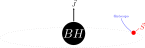
\includegraphics[scale=0.9]{images/solucion-en-kerr.pdf}
\caption[Solución helicoidal en Kerr]{Representación esquemática del sistema agujero negro-dipolo.}
\label{fig:7}
\end{figure}

Al ser un movimiento circular, usando coordenadas $x^{\mu}=[t,r,\theta,\phi]$, asumimos una 4-velocidad de la forma
\begin{equation}
\label{u}
u^{\mu} = \left[ \gamma, \  0, \  0, \  \omega \gamma \right],
\end{equation}
donde $\omega$ es la velocidad angular de la órbita y se define
\begin{equation}
\gamma:= \sqrt{ \frac{R}{R - 2m - 2 a^{2} m \omega^{2} - a^{2} \omega^{2} R + 4 a m \omega - \omega^{2} R^{3}}},
\end{equation}
donde $R$ es el radio de la órbita y $m,a$ son los parámetros del agujero negro. En un espaciotiempo plano $ \gamma $ se reduce al factor de Lorentz.

También consideraremos que la dirección del espín es paralela al momento angular del agujero negro, es decir que $S^{\mu} = \left[ 0,0,S^{\theta},0 \right]$.

De \eqref{eq:44} notamos que, al considerar la condición suplementaria de Mathisson-Pirani, la forma del 4-momentum puede ser escrita como
\begin{equation}
\label{p}
p^{\mu} =  M u^{\mu} - a_{\nu} S^{\mu \nu}, 
\end{equation}
donde $M:= p^{\mu} u_{\mu}$ es la masa del giróscopo y $a_{\nu}$ la 4-aceleración del giróscopo definida como $a_{\mu} := \delta u_{\mu} / \mathrm{d} s$.

De \eqref{u} calculamos la 4-aceleración del giróscopo, obteniendo que
\begin{equation}
\label{acceleration}
a^{\mu} = \left[ 0, \  - \frac{\gamma^2 \Theta}{R^6} \left(a^{2} - 2 m R + R^{2}\right), \  0, \  0\right],
\end{equation}
donde
\begin{equation}
\label{Theta}
\Theta := R^{2} \left( a^{2} m \omega^{2} - 2 a m \omega + m - \omega^{2} R^{3}\right).
\end{equation}

Luego, reemplazando \eqref{spintensor}, \eqref{u} y \eqref{acceleration} en \eqref{p}, tenemos que el 4-momentum es
\begin{align}
\label{mom5}
p^{\mu} &= \left[ \gamma M + \frac{\gamma^3 S^{\theta} \Theta}{R^6}  \left( a m - 2 a^{2} \omega m + a^{2}\omega R + \omega R^{3}\right), \  0, \  0, \ \gamma M \omega  - \frac{\gamma^3 S^{\theta} \Theta}{R^6} \left( 2 a m \omega - 2 m + R \right)\right].
\end{align}

Al trabajar el problema en coordenadas pseudo-esféricas esperamos que el 4-momentum sea un 4-vector constante respecto al parámetro de la curva, es decir que $\mathrm{d} p^{\mu} / \mathrm{d}s  = 0$, de esta forma tenemos que \eqref{eq:82} se reduce a
\begin{equation}
\label{dp}
R_{\nu \gamma \rho}^{\ \ \ \mu} S^{\nu \gamma} u^{\rho} + 2 \Gamma^{\mu}_{\rho \sigma} p^{\rho} u^{\sigma} = 0.
\end{equation}

Luego de reemplazar \eqref{spintensor}, \eqref{u} y \eqref{mom5} in \eqref{dp}, resolvemos $S$ en términos de $M$, $R$ y $\omega$, obteniendo que
\begin{equation}
\label{spinvalue}
S^{\theta} = \frac{M}{\gamma^2}\frac{\Theta}{\Upsilon},
\end{equation}
donde
\begin{align}
\Upsilon &:= 5 a^{5} m^{2} \omega^{4} + 3 a^{5} m \omega^{4} R - 20 a^{4} m^{2} \omega^{3} - 6 a^{4} m \omega^{3} R + 3 a^{3} m^{2} \omega^{4} R^{2} + 30 a^{3} m^{2} \omega^{2} \nonumber \\
& \quad + 7 a^{3} m \omega^{4} R^{3} - 9 a^{2} m^{2} \omega^{3} R^{2} - 20 a^{2} m^{2} \omega - 12 a^{2} m \omega^{3} R^{3} + 6 a^{2} m \omega R + 9 a m^{2} \omega^{2} R^{2} \nonumber \\
& \quad + 5 a m^{2} + 6 a m \omega^{4} R^{5} + 3 a m \omega^{2} R^{3} - 3 a m R - 3 m^{2} \omega R^{2} - 6 m \omega^{3} R^{5} + 2 m \omega R^{3} + \omega^{3} R^{6}.
\end{align}

Finalmente, si se substituye \eqref{spinvalue} en \eqref{mom5}, los valores del 4-momentum y 4-espin son, respectivamente,
\begin{align}
p^{\mu} &= \left[ \frac{M}{\gamma}\frac{\Lambda}{\Upsilon},\ 0,\ 0, \frac{M}{\gamma}\frac{\Omega}{\Upsilon} \right], \label{momentum} \\
S^{\mu} &= \left[ 0, \  0, \frac{M}{\gamma^2}\frac{\Theta}{\Upsilon} , \  0\right], \label{spin}
\end{align}
donde $\Lambda$ y $\Omega$ son funciones que dependen solamente de los parámetros de la órbita, dados por
\begin{align}
\Lambda &:= a^{4} m^{2} \omega^{3} - 3 a^{3} m^{2} \omega^{2} - 3 a^{3} m \omega^{2} R + 3 a^{2} m^{2} \omega - 2 a^{2} m \omega^{3} R^{3} + 6 a^{2} m \omega R - a m^{2} \nonumber \\
& \quad  - 3 a m R  + 2 m \omega R^{3} + \omega^{3} R^{6}
,\\
\Omega &:=  m \left(1-a \omega\right) \left(- a^{2} m \omega^{2} + 3 a^{2} \omega^{2} R + 2 a m \omega - 3 a \omega R - m + 4 \omega^{2} R^{3}\right).
\end{align}

Los siguientes invariantes son calculados también:
\begin{align}
a^{\mu} a_{\mu} &= -\frac{\gamma^4 \Theta^2}{R^{10}}\left( a^{2} - 2 m R + R^{2}\right), \label{aa}\\
S^{\mu} S_{\mu} &= - \frac{M^{2} \Theta^{2} R^{2}}{\Upsilon^{2} \gamma^{4}}, \\
\label{momentumnorm}
p^{\mu} p_{\mu} &= - \frac{M^{2} \left(2 \Lambda^{2} m - \Lambda^{2} R - 4 \Lambda \Omega a m + 2 \Omega^{2} a^{2} m + \Omega^{2} a^{2} R + \Omega^{2} R^{3}\right)}{\gamma^{2} \Upsilon^{2} R}. 
\end{align}

\section{Propiedades de la solución}

Estamos interesados en estudiar la norma del 4-momentum en términos de la velocidad angular a fin de encontrar valores de $\omega$ donde el 4-momentum sea un vector tipo tiempo. Primero buscamos valores de $\omega$ para los cuales \eqref{momentumnorm} es cero, esto es una ecuación polinomial de grado 8 para $\omega$, incluyendo un factor cuadrático proveniente de $\gamma^{-2}$ en \eqref{momentumnorm}. Esto determina dos raíces analíticas, dadas por
\begin{equation}
\omega_{\mathrm{min}} = \frac{2 a m - R \sqrt{a^{2} - 2 m R + R^{2}}}{2 a^{2} m + a^{2} R + R^{3}}, \quad \omega_{\mathrm{max}} = \frac{2 a m + R \sqrt{a^{2} - 2 m R + R^{2}}}{2 a^{2} m + a^{2} R + R^{3}}, \label{eq:omega}
\end{equation}
para los que $\gamma^{-2}$ es cero, y representan los valores mínimos y máximos de $\omega$ tales que $\gamma$ es real. Así, se asegura que la 4-velocidad $u^{\mu}$ es un vector tipo tiempo si $\omega_{\mathrm{min}} < \omega < \omega_{\mathrm{max}}$.

Más aún, cuando  $ \omega = \omega_ {\mathrm{min}} $, o bien cuando $\omega = \omega_\mathrm{max}$, podemos observar que  $ p^{\mu} p_{\mu} \to 0$ y $S^{\mu} S_{\mu} \to 0 $, mientras que la 4-aceleración $ a^{\mu} a_{\mu} \to - \infty $. Este comportamiento es producto de que para tales valores de velocidad angular, la velocidad del giróscopo tiende a la velocidad de la luz.

Introduciendo las variables adimensionales 
\begin{align}
\bar{R} &:= \frac{R}{m},\\
\bar{a} &:= \frac{a}{m},\\
\bar{\omega} &:= \omega m,
\end{align}
podemos reescribir \eqref{eq:omega} como
\begin{equation}
\bar{\omega}_{\mathrm{min}} = \frac{2 \bar{a} - \bar{R} \sqrt{\bar{R}^{2} - 2 \bar{R} + \bar{a}^{2}}}{2 \bar{a}^{2} + \bar{a}^{2} \bar{R} + \bar{R}^{3}},
\quad 
\bar{\omega}_{\mathrm{max}} = \frac{2 \bar{a} + \bar{R} \sqrt{\bar{R}^{2} - 2 \bar{R} + \bar{a}^{2}}}{2 \bar{a}^{2} + \bar{a}^{2} \bar{R} + \bar{R}^{3}},
\end{equation}
mientras que la normal del 4-momentum puede ser reescrita como
\begin{equation}
\label{ppadimentional}
\bar{p}^{\mu} \bar{p}_{\mu} := \frac{p^{\mu} p_{\mu}}{M^2} = - \frac{2 \bar{\Lambda}^{2} - \bar{\Lambda}^{2} \bar{R} - 4 \bar{\Lambda} \bar{\Omega} \bar{a} + 2 \bar{\Omega}^{2} \bar{a}^{2} + \bar{\Omega}^{2} \bar{a}^{2} \bar{R} + \bar{\Omega}^{2} \bar{R}^{3}}{\gamma^{2} \bar{\Upsilon}^{2} \bar{R}},
\end{equation}
donde
\begin{align}
\bar{\Lambda} &:= \frac{\Lambda}{m^3} = \bar{R}^{6} \bar{\omega}^{3} - 2 \bar{R}^{3} \bar{\omega}^{3} \bar{a}^{2} + 2 \bar{R}^{3} \bar{\omega} - 3 \bar{R} \bar{\omega}^{2} \bar{a}^{3} + 6 \bar{R} \bar{\omega} \bar{a}^{2} - 3 \bar{R} \bar{a} + \bar{\omega}^{3} \bar{a}^{4} \nonumber \\
& \qquad \qquad  - 3 \bar{\omega}^{2} \bar{a}^{3} + 3 \bar{\omega} \bar{a}^{2} - \bar{a},\\
\bar{\Omega} &:=  \frac{\Omega}{m^2} = \left(1 - \bar{\omega} \bar{a} \right) \left(4 \bar{R}^{3} \bar{\omega}^{2} + 3 \bar{R} \bar{\omega}^{2} \bar{a}^{2} - 3 \bar{R} \bar{\omega} \bar{a} - \bar{\omega}^{2} \bar{a}^{2} + 2 \bar{\omega} \bar{a} - 1\right),\\
\bar{\Upsilon} &:= \frac{\Upsilon}{m^3} = \bar{R}^{6} \bar{\omega}^{3} + 6 \bar{R}^{5} \bar{\omega}^{4} \bar{a} - 6 \bar{R}^{5} \bar{\omega}^{3} + 7 \bar{R}^{3} \bar{\omega}^{4} \bar{a}^{3} - 12 \bar{R}^{3} \bar{\omega}^{3} \bar{a}^{2} + 3 \bar{R}^{3} \bar{\omega}^{2} \bar{a} + 2 \bar{R}^{3} \bar{\omega} 
 \nonumber \\
& \qquad \qquad + 3 \bar{R}^{2} \bar{\omega}^{4} \bar{a}^{3} - 9 \bar{R}^{2} \bar{\omega}^{3} \bar{a}^{2} + 9 \bar{R}^{2} \bar{\omega}^{2} \bar{a} - 3 \bar{R}^{2} \bar{\omega} + 3 \bar{R} \bar{\omega}^{4} \bar{a}^{5} - 6 \bar{R} \bar{\omega}^{3} \bar{a}^{4} + 6 \bar{R} \bar{\omega} \bar{a}^{2} \nonumber\\
& \qquad \qquad - 3 \bar{R} \bar{a} + 5 \bar{\omega}^{4} \bar{a}^{5} - 20 \bar{\omega}^{3} \bar{a}^{4} + 30 \bar{\omega}^{2} \bar{a}^{3} - 20 \bar{\omega} \bar{a}^{2} + 5 \bar{a},\\
\gamma &= \sqrt{ \frac{\bar{R}}{\bar{R} - 2 - 2 \bar{a}^{2}  \bar{\omega}^{2} - \bar{a}^{2} \bar{\omega}^{2} \bar{R} + 4 \bar{a}  \bar{\omega} - \bar{\omega}^{2} \bar{R}^{3}}},
\end{align}

El comportamiento general de $p^{\mu}p_{\mu}$ se muestra en las figuras \ref{fig:2} y \ref{fig:3}. Vemos que existen dos raíces adicionales para los cuales \eqref{ppadimentional} se hace 0 dentro del intervalo $\bar{\omega}_{\mathrm{min}} < \bar{\omega} < \bar{\omega}_{\mathrm{max}}$. Las expresiones analíticas para tales raíces son complicadas de escrbir, y no las mostraremos aquí, pero nos referiremos a ellas como $\bar{\omega}_-$ y $\bar{\omega}_+$. El 4-momentum es siempre un vector tipo espacio cuando $\omega$ es un valor dentro del intervalo $\bar{\omega}_- < \bar{\omega} < \bar{\omega}_+$. El hecho de que el 4-mometum se asuma como un vector tipo tiempo significa probablemente que para tales valores de $\omega$ la aproximación polo-dipolo ya no es válida. Por ejemplo, si $\bar{R} = 5$ tenemos que los valores máximos/mínimos para la velocidad angular son $\bar{\omega}_{\mathrm{min}} \approx -0.155$, $\bar{\omega}_{\mathrm{max}} \approx 0.155$ y $\bar{\omega}_{\pm} \approx \pm 0.02$. Para órbitas lejos del agujero de negro, por ejemplo $\bar{R} = 10$, tenemos que $\bar{\omega}_{\mathrm{min}} \approx -0.089$, $\bar{\omega}_{\mathrm{max}} \approx 0.089$ and $\bar{\omega}_{\pm} \approx \pm 0.005$.

Note que en un espaciotiempo de Minkowski el 4-momentum es siempre un vector tipo tiempo. En la métrica de Schwarzschild $\bar{p}^{\mu}\bar{p}_{\mu}$ tiene una divergencia para $ \bar{\omega} =  0 $, ver figura \ref{fig:2}. Esto es porque el 4-momentum, como podemos ver en \eqref{p}, se construye a partir de un término cinético usual y otro proporcional al espín del cuerpo. Mientras que el 4-momentum cinético se mantiene finito en este caso, el espín diverge, tal y como se puede ver de \eqref{spinvalue} ya que $\bar{\Upsilon}$ se anula.

\begin{figure}[!ht]
\centering
\begin{subfigure}{0.45\textwidth}
\includegraphics[width=\textwidth]{images/grafico-schwarzschild}
\caption{$\bar{a}=0$}
\label{fig:2}
\end{subfigure}
\begin{subfigure}{0.45\textwidth}
\includegraphics[width=\textwidth]{images/grafico-kerr}
\caption{$\bar{a}=1/2$}
\label{fig:3}
\end{subfigure}
\caption[Norma del 4-momentum en espaciotiempo curvo]{\small{Norma del 4-momentum y 4-espín para los valores adimensionales $\bar{R} = 5$.}}
\end{figure}

De forma similar, en un espaciotiempo de Kerr el comportamiento de $\bar{p}^{\mu} \bar{p}_{\mu}$ es muy parecido al caso en la métrica de Schwarzschild, tal y como se observa en la figura \ref{fig:3}, pero ahora las velocidades angulares se encuentran desplazadas producto de la rotación del agujero negro. Ahora el valor de $\bar{\omega}$ para el que $S$ y $\bar{p}^{\mu} \bar{p}_{\mu}$ diverge ya no es cero. Por ejemplo, para $\bar{R} = 5$ y $\bar{a} = 1/2$, la velocidad angular mínima/máxima del giróscopo es $\bar{\omega}_{\mathrm{min}} \approx -0.146$ y $\bar{\omega}_{\mathrm{max}} \approx 0.162$, respectivamente.

Además, el valor del espín se indetermina para $ \bar{\omega} \approx 0.027 $ ya que, para este set de parámetros, es una raíz de $\bar{\Upsilon}$. Nos referiremos a este valor como \textit{velocidad angular crítica}. Es interesante que incluso para $ \bar{\omega} = 0 $ existen órbitas circulares para las cuales el 4-momentum es un vector tipo tiempo, no así en el caso en Schwarzschild. Así mismo, para tales parámetros tenemos que $\bar{\omega}_- \approx 0.007$ y $\bar{\omega}_+ \approx 0.04$. De esta forma, concluimos que para velocidades angulares cercanas al valor crítico dado por $ \bar{\omega} \approx 0.027 $, es decir, dentro de intervalo $ \bar{\omega}_- < \bar{\omega} < \bar{\omega}_+$, la aproximación polo-dipolo ya no es válida.

\section{Casos particulares}

A partir de la solución mostrada en \eqref{momentum} y \eqref{spin} podemos estudiar el comportamiento de un giróscopo para casos particulares más simples. Por ejemplo, si consideramos el caso de un giróscopo estático, es decir imponiendo $\omega = 0$, los valores de 4-momentum, 4-espín y 4-aceleración son, respectivamente,
\begin{align}
p^{\mu} &= \left[ \frac{M \left(3 R + m\right)}{\gamma \left(3 R - 5 m\right)},\  0,\  0,\  \frac{M m}{\gamma a \left(3 R - 5 m\right)} \right],\\
S^{\mu} &= \left[ 0,\ 0,\ \frac{M R^{2}}{\gamma^{2} a \left(3 R - 5 m\right)},\ 0 \right],\\
a^{\mu} &= \left[ 0, -\frac{m \left(a^{2} - 2 m R + R^{2}\right)}{R^{3} \left(2 m - R\right)}, \ 0, \ 0  \right],
\end{align}
donde $\gamma = \sqrt{1/(1-2m/R)}$.

Los siguientes invariantes también son calculados
\begin{align}
p^{\mu} p_{\mu} &= \frac{M^{2} \left(- 2 m + R\right) \left(- 12 a^{2} m + 9 a^{2} R - m^{2} R\right)}{a^{2} \left(- 5 m + 3 R\right)^{2}},\\
S^{\mu} S_{\mu} &= - \frac{M^{2} R^{4} \left(2 m - R\right)^{2}}{a^{2} \left(5 m - 3 R\right)^{2}},\\
a^{\mu} a_{\mu} &= \frac{m^{2} \left(- a^{2} + 2 m R - R^{2}\right)}{R^{4} \left(2 m - R\right)^{2}},
\end{align}
de donde se puede observar una clara divergencia cuando $a \to 0$. Esto es esperable ya que, como dijimos anteriormente, para el caso de la métrica de Schwarszchild existe una divergencia para $\omega = 0$. Es interesante hacer notar que si definimos la 4-fuerza sobre el giróscopo como
\begin{equation}
\label{eq:124}
F_{\mu} := M a_{\mu} = \left[ 0,  M \frac{m}{R\left( 2m-R \right)} , 0, 0 \right],
\end{equation}
y si consideramos el caso asintótico, es decir $R \gg m $, entonces la expresión anterior se reduce a la ley de gravitación universal
\begin{equation}
\vb{F} \approx -\frac{mM}{R^2} \hat{r} = -\left( \frac{GM}{R^2} M_{\mathrm{BH}} \right) \hat{r},
\end{equation}
donde $M_{\mathrm{BH}}$ es la masa del agujero negro. Esto es evidente puesto que el sistema en cuestión representa el movimiento de un masa de prueba alrededor de un cuerpo central.

Otro caso importante de destacar es cuando la velocidad angular del cuerpo viene dada por
\begin{equation}
\omega =\omega_{\mathrm{g} \pm} = \frac{1}{a \pm \sqrt{\frac{R^3}{m}}},
\end{equation}
y representa la velocidad angular de trayectorias geodésicas circulares. Para este caso el valor del espín es cero, lo cual es esperable para la dinámica de una partícula monopolar.

Podemos deducir, a partir de \eqref{momentum} y \eqref{spin}, la solución a un problema equivalente en la métrica de Minkowski con el límite $m \to 0$, encontrando que
\begin{align}
\label{eq:27}
p^{\mu} &= \left[  \frac{M}{\gamma},\ 0,\ 0,\ 0 \right],\\
\label{eq:28}
S^{\mu} &= \left[\ 0,\ 0,\ -\frac{M}{\gamma^2 v}, \ 0 \right],\\
\label{eq:acent}
a^{\mu} &= \left[ \ 0,\ -\gamma^2  \omega^2 R,\ 0,\ 0 \right],
\end{align}
donde $\gamma = 1/\sqrt{1-v^2}$ y $v$ es la velocidad tangencial del giróscopo. 

De \eqref{eq:acent} podemos observar la aceleración centrípeta del cuerpo, ya que este sigue un movimiento circular. Por otro lado, y como es de esperar, el 4-momentum es siempre un 4-vector tipo tiempo, mientras que la norma del 4-espín obedece que
\begin{equation}
\label{eq:78}
S_{\mathrm{M}} :=  \sqrt{- S^{\mu} S_{\mu}} = \frac{MR}{\gamma^2_{\mathrm{K}}v}.
\end{equation}

Estos resultados concuerdan con los presentados en \cite{Costa-Herdeiro-Natario-Zilhao} donde órbitas circulares en la métrica de Minkowski son estudiadas bajo la condición suplementaria de Mathisson-Pirani y es discutida su interpretación física.

Otro caso a destacar se muestra cuando la velocidad angular del cuerpo es
\begin{equation}
\omega = \frac{a}{a^2+R^2},
\end{equation}
ya que como se puede ver en \cite{Costa-Natario-Zilhao}, para órbitas circulares en el plano ecuatorial con tal velocidad angular todas las componentes del tensor gravito-magnético de mareas son cero, por lo que se satisface que
\begin{equation}
\label{eq:higual0}
\cd{p^{\mu}}  = 0.
\end{equation}

La expresión anterior quiere decir que un giróscopo siguiendo una trayectoria circular con tal velocidad angular específica en un espaciotiempo de Kerr no experimentará ningún cambio en su dinámica producto de fuerzas de marea. Algo similar ocurre en la teoría electromagnética con un dipolo magnético siguiendo una órbita circular alrededor de una carga central $Q$ con momento magnético $\mu_{\mathrm{s}}$, en este caso no es posible anular todas las componentes del tensor magnético de mareas puesto que sus componentes no-nulas son, en el plano ecuatorial, vienen dadas por
\begin{align}
\mathtt{B}_{r \theta} &= \alpha \left( r^2 Q u^{\phi} - 3\mu_s u^t \right),\\
\mathtt{B}_{\theta r} &= \alpha \left( 2r^2 Q u^{\phi} - 3\mu_s u^t \right),\\
\mathtt{B}_{r \phi} &= -\alpha Q r^2 u^{\theta},\\
\mathtt{B}_{\phi r} &= -2\alpha Q r^2 u^{\theta,}\\
\mathtt{B}_{t r} &= 3 \alpha \mu_s u^{\theta},\\
\mathtt{B}_{t \theta} &= 3 \alpha \mu_s u^{r},
\end{align}
donde $\alpha = 1/r^3$.

Imponiendo una velocidad angular de la forma
\begin{equation}
\label{eq:angular-velocity-em}
\omega = 2 \frac{\mu_s}{Q r^2},
\end{equation}
el tensor de mareas se reduce a su parte antisimétrica $\mathtt{B}_{\mu \nu} = \mathtt{B}_{[\mu \nu]}$. De esta forma, un dipolo magnético siguiendo una trayectoria con tales características siempre experimentará una fuerza producto del campo externo, lo que marca una clara diferencia entre Relatividad General y la teoría electromagnética clásica causada por los efectos de inducción magnética. Para más información ver Ref. \cite{Costa-Herdeiro-Natario-Zilhao}.

De \eqref{eq:higual0} se obtiene que los siguientes valores para el 4-momentum, 4-espín y 4-aceleración son, respectivamente,
\begin{align}
\label{eq:ssc-mp-p}
p^{\mu} &= \frac{1}{\sqrt{R^2 + a^2 - 2mR}} \left[ M (m + R), 0, 0, \frac{M m}{a} \right],\\
\label{eq:ssc-mp-s}
S^{\mu} &= \left[ 0, 0, - \frac{MR}{a}, 0 \right],\\
a^{\mu} &= \left[ 0, \ \frac{- a^{2} + m R}{R^{3}}, \  0, \  0\right],
\end{align}
donde además la 4-velocidad del giróscopo es
\begin{equation}
\label{eq:4-velocitiy-helical}
u^{\mu} = \frac{1}{\sqrt{R^4 + a^2 R^2 - 2mR^3}} \left[ a^2 + R^2, 0, 0, a \right].
\end{equation}

Note que para $ a \to 0 $ se tiene que $ | S^{\theta} | \to \infty $, esto es causado por el hecho que $ \omega \propto a $ y como $ a \to 0 $ entonces el cuerpo tiende a mantenerse estático respecto del agujero negro y, como vimos anteriormente, este es un caso que presenta una divergencia cuando $\omega=0$.

Como es de esperar, y al igual que en el caso con $\omega=0$ en la métrica de Kerr, la 4-fuerza sobre el giróscopo es
\begin{equation}
\label{eq:124}
F_{\mu} = \left[ 0, \frac{M(a^2 - mR)}{R\left( a^2 - 2mR + R^2  \right)},0,0 \right],
\end{equation}
que al considerar el caso asintótico se obtiene, como es de esperar, la ley de gravitación universal de Newton
\begin{equation}
\vb{F} \approx -\frac{mM}{R^2} \hat{r} = -\left( \frac{GM}{R^2} M_{\mathrm{BH}} \right) \hat{r},
\end{equation}
donde $M_{\mathrm{BH}}$ es la masa del agujero negro, ya que nuevamente, esta situación representa el caso de un masa de prueba estática respecto al cuerpo central.

Para este caso podemos observar además que el 4-momentum del giróscopo es siempre un vector tipo espacio fuera del horizonte de eventos, ya que
\begin{equation}
p^{\mu} p_{\mu} = -\frac{M^{2} R^{2} \left(m^2 - a^2\right)}{a^{2} \left(R^{2} - 2 R m + a^{2}\right)}.
\end{equation}

El hecho de que el 4-momentum generalmente se asume como un vector temporal significa que en este caso ya no sería válida la descripción a orden dipolar.